\documentclass[12pt]{report} % Use report class for chapters
\usepackage[a4paper, margin=1in]{geometry} % Adjust margins
\usepackage{amsmath, amssymb} % For math formatting
\usepackage{titlesec} % For customising section titles
\usepackage{fancyhdr} % For headers and footers
\usepackage{hyperref} % For a clickable table of contents and references
\usepackage{tocloft} % For customising the table of contents
\usepackage{setspace} % For line spacing

% Formatting title sections
\titleformat{\chapter}[hang]{\bfseries\LARGE}{Chapter \thechapter}{1em}{}
\titleformat{\section}[hang]{\large\bfseries}{\thesection}{1em}{}

% Customise TOC spacing
\renewcommand{\cftchapdotsep}{1.5} % Adjust dots in TOC

% Line spacing
\onehalfspacing % Set 1.5 line spacing

% Header and footer
\pagestyle{fancy}
\fancyhf{}
\fancyhead[L]{\slshape \leftmark} % Chapter title on left
\fancyfoot[C]{\thepage} % Page number at center

% Math and Symbols
\usepackage{amsmath, amssymb} % For math environments and symbols

% Graphics and Floats
\usepackage{graphicx} % Include images
\usepackage{float} % Improved float handling

% Hyperlinks
\usepackage{hyperref} % For clickable hyperlinks

% Code Listings
\usepackage{listings} % For code formatting
\usepackage{xcolor} % For color definitions

% Citations
\usepackage[numbers, super]{natbib} % For citation styles
% Remove \usepackage{cite}, as natbib replaces it.

% Title Page
\title{Ridge Regression for S\&P 500 Analysis}
\author{Raul Unnithan}
\date{\today}

\begin{document}
\maketitle

\tableofcontents

\chapter{Introduction}
\section{Background}
High-dimensional data refers to data in which the number of variables, $p$, is much larger than the number of observations, $n$.\cite{reza2024} It is increasingly common in various fields, such as finance, genomics, and social sciences. Analysing high-dimensional data poses issues, mainly due to over-fitting, multicollinearity and identifying the most relevant subset of variables.\cite{reza2024} Multicollinearity is an issue because it makes it difficult to tell which predictor is impacting the response variable. Ridge regression is a penalised regression technique which solves these problems by incorporating a penalty term that reduces the impact of less important variables, thus shrinking their coefficients towards zero without removing them from the model.\cite{hailiang2023}

\section{Research Objectives and Aims}
This report applies Ridge Regression to an S\&P 500 dataset to identify the key stocks influencing average market returns. It simplifies the model and shrinks irrelevant features through the $L_2$ penalty: \(\|\boldsymbol{\beta}\|_2^2 = \sum_{j=1}^{p} \beta_j^2\). The larger coefficients in the Ridge model represent the more influential stocks, which significantly impact overall returns. Cross-validation optimises the regularisation parameter ($\lambda$), thus balancing model simplicity and predictive accuracy by minimising Mean Squared Error (MSE). The report also uses a coefficient path to understand how the estimated coefficients of the Ridge regression model change as the regularisation parameter changes.

\section{Literature Review}
The curse of dimensionality is prevalent in financial modelling, where datasets can involve hundreds of predictors. Fan and Li (2001) highlighted the limitations of Ordinary Least Squares (OLS)-based variable selection methods in such cases because these selection procedures ignore random errors inherited in each variable selection stage. \cite{fanli2001} 

Tikhonov (1943) introduced Ridge regression to solve this by incorporating a penalty term, shrinking coefficients toward zero while keeping all predictors in the model.\cite{hailiang2023} Hoerl and Kennard (1970) established the theory for Ridge regression, demonstrating its superiority over OLS in multi-collinear data by introducing a bias term, reducing the variance of the estimators.\cite{hoerlken1970} 

Ridge regression is used widely in financial research. Giannone (2016) highlighted Ridge regression's Bayesian foundation by demonstrating its predictive accuracy and extending it beyond simple forecasts, demonstrating its effectiveness in high-dimensional financial datasets.\cite{giannone2016} Ridge regression, despite its versatility in financial contexts like bond pricing, has a limited application to time series datasets like the S\&P 500 in current literature.

Existing studies, such as Sant'Anna (2020), have used Lasso regression to analyse index funds. Lasso handles variable selection better because it can set coefficients of irrelevant features completely to zero, unlike Ridge. However, its use of the $L_1$ parameter: $\|\boldsymbol{\beta}\|_1 = \sum_{i=1}^{n} | \beta_i |$ makes it less suitable for multi-collinear datasets like S\&P 500, as it excludes some predictors. The S\&P 500 is multi-collinear because all these stocks can be affected by substantial global events such as recessions. This report addresses gaps in Ridge regression analysis by using its improved ability to handle multicollinearity and identify influential stocks that have the most impact on average market returns.

\section{Ridge Regression}
\subsection{Theory}
Ridge regression is a linear regression method that includes a penalty term to constrain coefficient size.\cite{hailiang2023} Its objective function general form is:
\[
\boldsymbol{\hat{\beta}}_{\text{Ridge}} = \arg \min_{\boldsymbol{\beta}\in \mathbb{R}^p} \left\{ \|\boldsymbol{Y} - \boldsymbol{X\beta}\|_2^2 + \lambda \|\boldsymbol{\beta}\|_2^2 \right\}
\]
where \(\boldsymbol{\hat{\beta}}_{\text{Ridge}}\) is the vector of coefficient estimates,  
\(\boldsymbol{\beta}\) is the vector of regression coefficients,  
\(\boldsymbol{Y}\) is the response variable vector,  
\(\boldsymbol{X}\) is the matrix of predictor (feature) variables, with rows as observations and columns as predictors,  
the penalty term \(\|\boldsymbol{\beta}\|_2^2 = \sum_{j=1}^{p} \beta_j^2\) is the $L_2$ norm of \(\boldsymbol{\beta}\),  
and \(\lambda\) controls the trade-off between fit and coefficient magnitude, with larger values increasing the influence of the penalty. As $\lambda$ increases, the Ridge Regression model shrinks all coefficients toward zero, as shown in the coefficient path plot (Figure \ref{fig:Coefficient_Paths}).

The assumption that $\boldsymbol{\hat{\beta}}_{\text{Ridge}}$ minimises the general function can be shown by solving the above equation using differentiation with respect to $\boldsymbol{\beta}$, giving the closed-form estimator: $\boldsymbol{\hat{\beta}}_{\text{Ridge}} = \left( \mathbf{X}^T \mathbf{X} + \lambda \mathbf{I}_p \right)^{-1} \mathbf{X}^T \mathbf{Y}$.\cite{reza2024} This is the cost function Ridge Regression aims to minimise: 

\[
\|\boldsymbol{Y} - \boldsymbol{X\beta}\|_2^2 + \lambda \|\boldsymbol{\beta}\|_2^2 =
RSS + \lambda \boldsymbol{\beta}^T \boldsymbol{\beta}
\]


\noindent The second equality is expressing the residual sum of squares (RSS) as a matrix, which will be expanded upon and differentiated.

\begin{align*}
RSS + \lambda \boldsymbol{\beta}^T \boldsymbol{\beta} 
    &= (\mathbf{y} - \mathbf{X} \boldsymbol{\beta})^T (\mathbf{y} - \mathbf{X} \boldsymbol{\beta}) + \lambda \boldsymbol{\beta}^T \boldsymbol{\beta} \\
    &= \mathbf{y}^T \mathbf{y} - 2 \boldsymbol{\beta}^T \mathbf{X}^T \mathbf{y} + \boldsymbol{\beta}^T \mathbf{X}^T \mathbf{X} \boldsymbol{\beta} + \lambda \boldsymbol{\beta}^T \boldsymbol{\beta}
\end{align*}

\noindent Take the gradient with respect to $\boldsymbol{\beta}$ and set it to zero for the minimum:

\begin{align*}
-2 \mathbf{X}^T \mathbf{y} + 2 \mathbf{X}^T \mathbf{X} \boldsymbol{\beta} + 2 \lambda \boldsymbol{\beta} &= 0, \\
- \mathbf{X}^T \mathbf{y} + \mathbf{X}^T \mathbf{X} \boldsymbol{\beta} + \lambda \boldsymbol{\beta} &= 0, \\
\mathbf{X}^T \mathbf{X} \boldsymbol{\beta} + \lambda \boldsymbol{\beta} &= \mathbf{X}^T \mathbf{y}, \\
\left( \mathbf{X}^T \mathbf{X} + \lambda \mathbf{I} \right) \boldsymbol{\beta} &= \mathbf{X}^T \mathbf{y}, \\
\boldsymbol{\beta} &= \left( \mathbf{X}^T \mathbf{X} + \lambda \mathbf{I} \right)^{-1} \mathbf{X}^T \mathbf{y}.
\quad \hfill \blacksquare
\end{align*}

The $L_2$ penalty shrinks all coefficients toward zero without making them precisely zero, leading to simpler models that reduce multicollinearity and mitigate over-fitting.\cite{hailiang2023} This also leads to more stable models, especially when the number of variables is much larger than the number of observations.\cite{reza2024} Estimates from the ridge regression cost function, $ \|\boldsymbol{Y} - \boldsymbol{X\beta}\|_2^2 + \lambda \|\boldsymbol{\beta}\|_2^2$, solve the LS problem subject to the constraint $\sum_{j=1}^p \beta_j^2 \leq c$.\cite{hailiang2023} 

\noindent (Fletcher 2008) uses Karush-Kuhn Tucker (KKT) conditions to verify equivalence. It uses the Lagrangian along with this constraint to start the proof: \\ $
\mathcal{L}(\beta, \nu) = \| \mathbf{Y} - \mathbf{X}\beta \|_2^2 + \nu \left( \|\beta\|_2^2 - c \right),$ where \(\nu \geq 0\) is the Lagrange multiplier. 

The first KKT condition needs the Lagrangian gradient with respect to \(\beta\) to equal zero at the optimal solution:

\begin{align*}
    \frac{\partial \mathcal{L}}{\partial \beta} = -2\mathbf{X}^\top (\mathbf{Y} - \mathbf{X}\beta) + 2\nu\beta = 0, \\
(\mathbf{X}^\top \mathbf{X} + \nu \mathbf{I})\beta = \mathbf{X}^\top \mathbf{Y}.
\end{align*}

\noindent The second KKT condition is the complementarity property: $\nu (\|\beta\|_2^2 - c) = 0$, which has two consequences. If \(\nu > 0\), the constraint \(\|\beta\|_2^2 = c\) is active, meaning the solution lies on the constraint boundary, and if the constraint is inactive, i.e. (\(\|\beta\|_2^2 < c\)), then \(\nu = 0\), so the Lagrange multiplier is zero.\cite{fletcher2000practical} 

If \(\nu = \lambda\) and \(c = \|\hat{\beta}(\lambda)\|_2^2\), then the ridge estimator \(\hat{\beta}(\lambda)\) satisfies both KKT conditions, and both forms produce the same solution here.\cite{fletcher2000practical} \quad $\blacksquare$

The constraint defines a smooth $L_2$ ball in the coefficient space. This smooth constraint means that Ridge does not completely zero coefficients.\cite{hailiang2023} 


\section{Application}
\subsection{Dataset Processing and Analysis}
The high-dimensional dataset for analysis comes from Mendeley Data.\cite{mendeleydata} This is the S\&P 500 dataset, which includes the daily closing prices of multiple stocks from the S\&P 500 index. Ridge regression can be applied to this dataset to select influential stocks and spot their trends. This work is helpful for portfolio managers because they can improve their equity asset allocation.

The first analysis stage was to replace \texttt{NA}s in the \texttt{returns\_data} with the column mean. Mean imputation minimises bias and preserves the underlying distributions. The features in the matrix \texttt{X} were standardised with the \texttt{scale()} function, so each feature has a mean of 0 and a standard deviation of 1 and helps $\lambda$ identify relevant features. The dataset is split so the Ridge regression model can be trained. The \texttt{glmnet} package is used in R to carry out the ridge regression implementation. The key steps were computing daily returns from stock prices, imputing missing values with column means, and standardising predictors. The ridge model and cross-validation determined the optimal \( \lambda \). The model's performance was evaluated on the test via the MSE, and a plot showed the highest contributing predictors.

\subsection{Results}
The MSE on the test set was \texttt{2.02e-07}, so the ridge model worked well. The top contributing predictors from Figure \ref{fig:Top10} were STZ (Constellation Brands Inc.), GNW (Genworth Financial), and DVN (Devon Energy Corp). The results are all positive, so these companies did well in this period. DVN had a significant increase in oil production, explaining its higher returns. STZ acquired one of its competitors, Grupo Modelo, thus, why its stock prices were higher.\cite{constellation2013} Lasso could apply better to this dataset because it can remove features by shrinking their coefficients to zero, but Ridge deals with multicollinearity better. The condition number gives the multicollinearity. It is the square root of the largest eigenvalue over the smallest eigenvalue.\cite{conditionnumber} A condition number over 30 means high multicollinearity, and the condition number here was \texttt{72.49}. The \texttt{best\_lambda} was \texttt{0.0666}, so, despite the high multicollinearity, ridge deals with it well. In the coefficient path plot, Figure \ref{fig:Coefficient_Paths}, the paths shrink to zero, which should not occur for Ridge. It occurs due to the \texttt{glmnet} package treating small coefficient values as zero. 

\chapter{Conclusion}
\section{Summary of Findings}
 Key findings from this application of Ridge Regression to a high-dimensional time series dataset included:
\begin{itemize}
    \item The Ridge regression achieving a low MSE of \(2.02 \times 10^{-7}\), so the ridge model has a high prediction accuracy despite high dimensionality.
    \item STZ (Constellation Brands Inc.), GNW (Genworth Financial), and DVN (Devon Energy Corp.) being identified as the top contributors, with STZ having the most significant coefficient contribution.
    \item A high condition number confirming severe multicollinearity and appropriate use of Ridge Regression rather than Lasso, but Ridge regression addresses this well with a low \(\lambda\) value.
\end{itemize}

\section{Implications for Future Research \& Ridge Comparison}
Future research into this area could look into different ways of integrating Ridge regression with other regression techniques to improve prediction accuracy. 
For instance, Gasparin et al. (2020) use an adaptive elastic-net regularisation approach, which is a combination of Lasso, adaptive Lasso, and elastic-net techniques, showing how integrating sparsity and regularisation can effectively improve index tracking.\cite{Shu2020} This was done using a tracking error, which indicates the portfolio tracks the benchmark closely.

Testing other shrinkage methods proved to be interesting. Lasso achieved an MSE of \(3.82 \times 10^{-7}\), which, while a good accuracy, was not as good as Ridge. However, what was most noteworthy was testing the elastic net regularisation technique. Elastic net combines ridge and lasso so it considers both. This produced an MSE of \(4.71 \times 10^{-7}\), which is higher than the ridge MSE, indicating that ridge is the best-performing simple shrinkage method on this dataset.

% Change bibliography numbering format
\makeatletter
\renewcommand\@biblabel[1]{#1.} % Change numbering style to 1.
\makeatother
\bibliographystyle{unsrt}
\bibliography{references}

\chapter{Appendix}
\section{R Code}
\begin{lstlisting}[language=R, breaklines=true, basicstyle=\ttfamily\small, columns=fullflexible]
install.packages("glmnet")
library(glmnet)

sp500_data <- read.csv("C:\\Users\\raula\\OneDrive\\Documents\\Durham\\4th Year\\High-Dimensional Statistics\\Mini Project Report\\Code\\sp500data.csv")

# Remove first row and first column - dates and stock tickers
sp500_data <- sp500_data[-1, -1]

# Compute daily returns: (current - previous price)/previous price
returns_data <- diff(as.matrix(sp500_data)) / as.matrix(sp500_data[-nrow(sp500_data), ])

# Replace NA values in returns_data with column mean
returns_data[is.na(returns_data)] <- sapply(returns_data, function(x) mean(x, na.rm = TRUE))

# Define target variable `y' as average return of stocks per time
y <- rowMeans(returns_data, na.rm = TRUE)

# Convert X to matrix form and standardise predictors
X <- as.matrix(returns_data)
X <- scale(X)

# Split data into training and test sets
train_index <- sample(1:nrow(X), 0.7 * nrow(X))  # 70% for training

X_train <- X[train_index, ]
y_train <- y[train_index]
X_test <- X[-train_index, ]
y_test <- y[-train_index]

ridge_model <- cv.glmnet(X_train, y_train, alpha = 0)
best <- ridge_model$lambda.min

# Fit the final Ridge model using best lambda on the training data
final_model <- glmnet(X_train, y_train, alpha = 0, lambda = best)

# Evaluate the model on the test set
predictions <- predict(final_model, s = best, newx = X_test)
mse <- mean((y_test - predictions)^2)

# Ridge Minimiser Proof Verification: Generate synthetic data
n <- 100  
p <- 10   

X <- matrix(rnorm(n * p), nrow = n, ncol = p)  # Random predictor matrix
beta_true <- rnorm(p)  # True coefficients
y <- X %*% beta_true + rnorm(n, sd = 0.5)  # response with noise

# Ridge regression closed-form estimator
lambda <- 1 
I <- diag(p)  

ridge_beta <- solve(t(X) %*% X + lambda * I) %*% t(X) %*% y

# Verify by comparing with the glmnet package
ridge_model <- glmnet(X, y, alpha = 0, lambda = lambda / n) # dividing by n scales lambda
ridge_beta_glmnet <- as.vector(coef(ridge_model, s=lambda/n))[-1]

cat("Closed-form Ridge Coefficients:\n", ridge_beta, "\n")
cat("GLMNet Ridge Coefficients:\n", ridge_beta_glmnet, "\n")

# Verifying constraint proof satisfies KKT: simulate data
n <- 50  # Number of observations
p <- 100 # Number of predictors

X <- matrix(rnorm(n * p), nrow = n, ncol = p)  # Design matrix
beta_true <- rnorm(p)                          # True coefficients

Y <- X %*% beta_true + rnorm(n)                # Response vector
lambda <- 10

# Ridge regression using the normal equation
ridge_solution <- function(X, Y, lambda) {
  p <- ncol(X)
  I <- diag(p)  # Identity matrix
  beta_hat <- solve(t(X) %*% X + lambda * I) %*% t(X) %*% Y
  return(beta_hat)}
  
beta_ridge <- ridge_solution(X, Y, lambda)

verify_kkt <- function(X, Y, beta, lambda, tolerance = 1e-6) {
  # 1. Gradient condition (stationarity)
  gradient <- -2 * t(X) %*% (Y - X %*% beta) + 2 * lambda * beta
  gradient_condition <- all(abs(gradient) < tolerance)
  
  # 2. Complementarity condition
  beta_norm_squared <- sum(beta^2)
  complementarity_condition <- abs(lambda * (beta_norm_squared - beta_norm_squared)) < tolerance
  
  # Both conditions must be satisfied
  all_conditions <- gradient_condition & complementarity_condition
  return(all_conditions)}

kkt_satisfied <- verify_kkt(X, Y, beta_ridge, lambda)
print(kkt_satisfied) # returns True


\end{lstlisting}

\section{Additional Data Visualisations}

\begin{lstlisting}[language=R, breaklines=true, basicstyle=\ttfamily\small, columns=fullflexible]
# Plot Ridge Coefficient Paths, highlighting the best lambda

plot(ridge_model$glmnet.fit, xvar = "lambda", label = FALSE)
abline(v = log(best), col = "red", lty = 2)
title(main = "Ridge Regression Coefficient Paths", line = 2.5)
\end{lstlisting}

\begin{figure}[H]
    \centering
    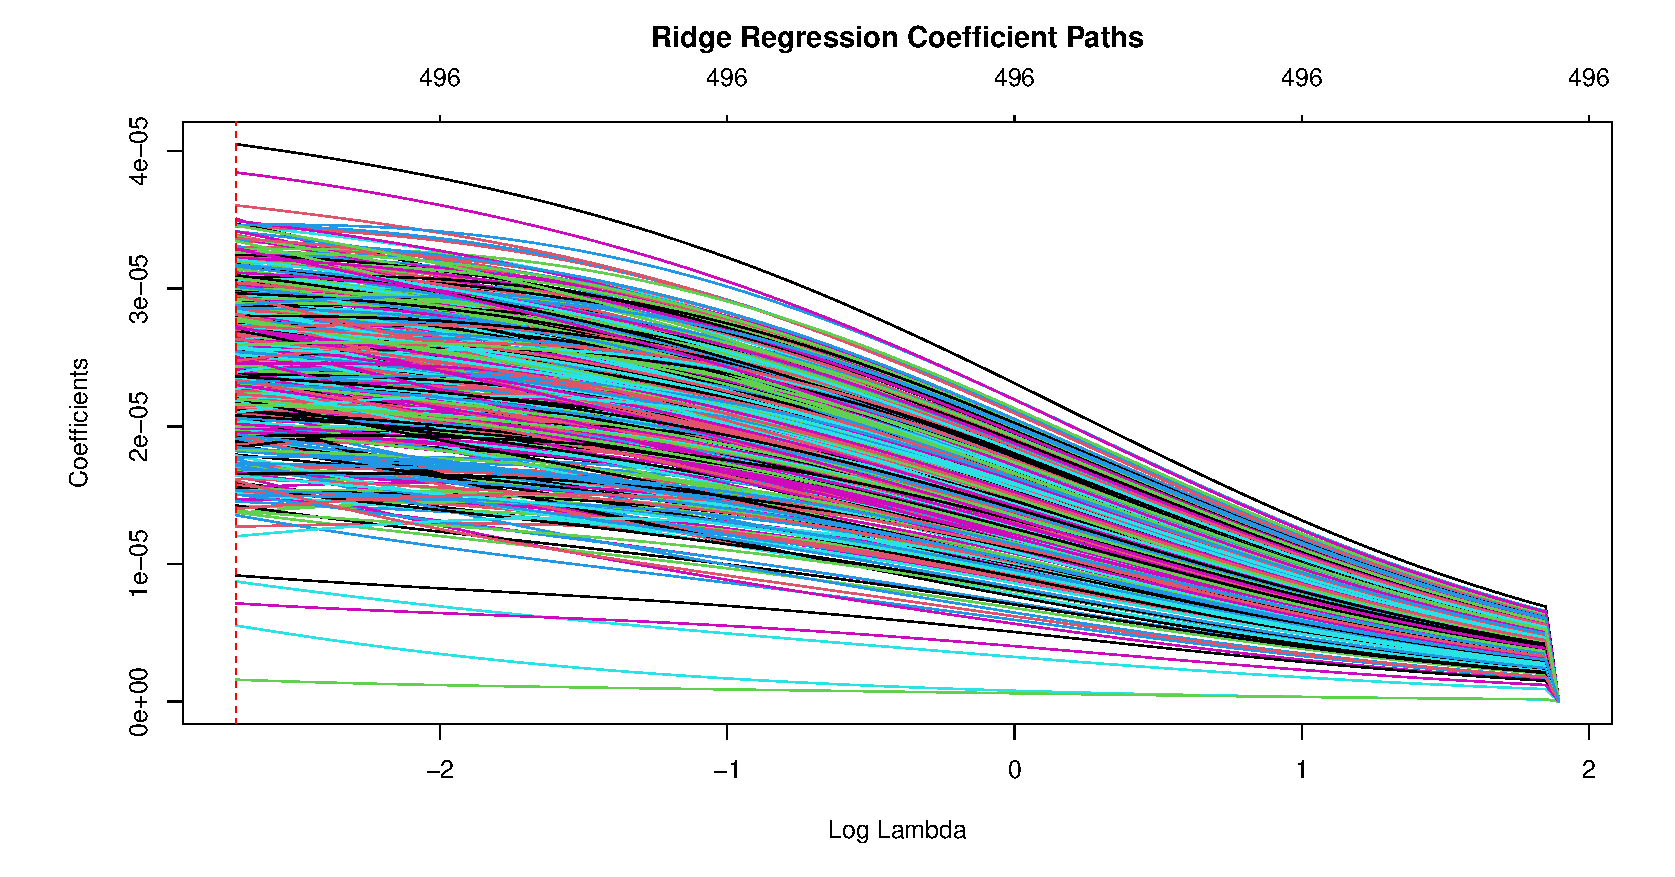
\includegraphics[width=0.8\textwidth]{Coefficient Paths.pdf}
    \caption{Ridge Coefficient Paths}
    \label{fig:Coefficient_Paths}
\end{figure}

\begin{lstlisting}[language=R, breaklines=true, basicstyle=\ttfamily\small, columns=fullflexible]
# Convert sparse matrix to a numeric vector and remove intercept
coefficients_vector <- as.numeric(coefficients)[-1]
# Assign correct stock names
names(coefficients_vector) <- rownames(coefficients)[-1]  

coefficients_vector <- coefficients_vector[!is.na(coefficients_vector) & is.finite(coefficients_vector)] # Remove invalid
top_10_coefs<-sort(abs(coefficients_vector),decreasing=TRUE)[1:10]
# Plot the top 10 coefficients
barplot(top_10_coefs, main = "Top 10 Stocks by Coefficient Magnitude (Excluding Intercept)", xlab = "Stocks", las = 2,  col = "steelblue", cex.names = 0.8)
\end{lstlisting}

\begin{figure}[H]
    \centering
    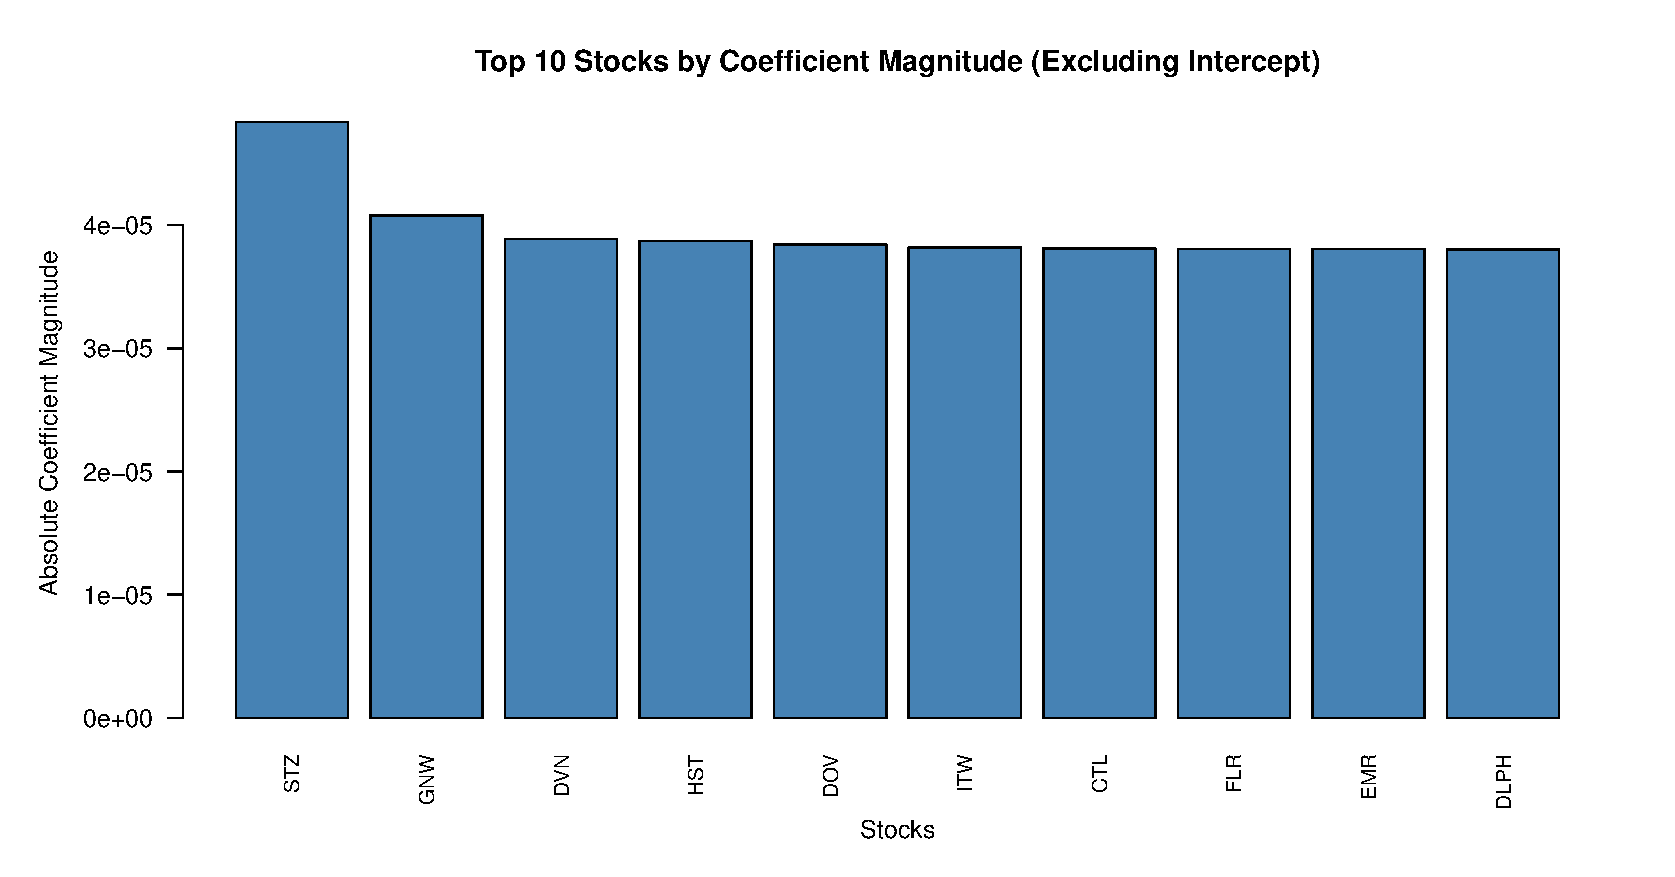
\includegraphics[width=0.8\textwidth]{Top10.pdf}
    \caption{Top 10 Contributing Stocks by Coefficient Magnitude}
    \label{fig:Top10}
\end{figure}

\end{document}
